
\section{Detection algorithm}
\label{sec:algorithm}

In case the search for signals is directed towards monotransits, the network outputs for a given input light curve can directly be used for detection. For example, one can set a threshold on peaks in the PTS, which can be considered as candidate detections. In case we wish to search for repeating signals, the RNN outputs alone are not enough. In order to compare the performance of an RNN-based detection algorithm with conventional methods such as BLS, we also need to determine the period and epoch of the signal. Two different algorithms are tested to do so, which only make use of the RNN outputs, i.e. the PTS, for a given input light curve. 

\subsection{PTS-Peak}
\label{sec:pts-peak}
As proposed by \cite{pearson2018searching}, one could use the distances between peaks in the PTS to determine the period of a repeating signal. Here we implement this idea and refer to the algorithm as PTS-Peak. In order for this algorithm to work well, we need to take into account the presence of potential false detections in the PTS, or multiple detections of signals belonging to different planets. Therefore we adopt several rules and filtering steps to ensure consistency between matched peaks and resulting parameter estimates. The algorithm we used takes the following steps:

\begin{enumerate}
    \item The PTS is smoothed using a one-dimensional Gaussian filter with a standard deviation of 9 data points, and peaks above a pre-set threshold are identified and indexed.
    \item For each peak $i$, the width of the peak above the threshold is used as candidate transit duration $\tau_i$ and the central point of the peak as candidate mid-transit time $t_{\text{mid},i}$. For each pair of peaks \{$i$, $j$\}, where $j>i$, the candidate period is determined by $P_{i,j} = t_{\text{mid},j} - t_{\text{mid},i}$.
    \item  For each pair of peaks \{$i$, $j$\}, a set is $c$ formed consisting of the indices of peaks that may correspond to signals from the same planet. The peak $k$ that has $t_{\text{mid},k}$ closest to time $t_{\text{exp}} = t_{\text{mid},j} + P_{i,j}$ is added to the candidate signal set $c=$ \{$i$, $j$\}, if $t_{\text{mid},k}$ is within three hours of $t_{\text{exp}}$. We then get the candidate $c=$ \{$i$, $j$, $k$\}, which is used to update the expected period, i.e. $P_{i,j,k} = (t_{\text{mid},k} - t_{\text{mid},i})/2$. Iteratively, the candidate set is expanded with the indices of peaks that lie within the expected range, until $t_{\text{exp}} - 3\text{h}$  is larger than the maximum time in the PTS. Candidate sets that have missing peaks at times where you would expect them are rejected and the rest is passed to the next step. Note that this would filter out detections if only a single peak is missing in the PTS. However, such signals can still be retrieved by evaluating the harmonics of a detected signal, as is described in step \ref{step:harmonics}.
    \item For each candidate $c$, the candidate duration $\tau_c$ is defined by the median duration of the individual peaks, the period $P_c$ by the median distance between peaks and the $t_{0,c}$ by the median of the epoch expected from subtracting $P_c$ from each individual $t_{\text{mid},i}$. A candidate is rejected if $\tau_c$ is smaller than 15 minutes or if $P_c < P_{\text{min}}$ for a pre-set minimum period $P_{\text{min}}$.
    \item\label{step:score} Each candidate is then given a score. For each individual event $n = \{0,\dots,E-1\}$ in the candidate signal defined by $t_{0,c}$, $\tau_c$ and $P_c$, i.e. $t_{0,c} + nP_c - \frac{1}{2}\tau_c< t < t_{0,c} + nP_c + \frac{1}{2}\tau_c$, the maximum in the PTS is recorded as $y_{n,\text{max}}$. The candidate score is then given by:
    \begin{equation}
        score = \frac{1}{\sqrt{E}}\sum_{n=0}^{E-1} y_{n,\text{max}},
    \end{equation}
    where the square root is used to prioritize detections with more individual events over detections with similar scores $y_{n,\text{max}}$, but fewer events. Only the best scoring candidate is passed to the next step.
    \item\label{step:harmonics}  Finally, the harmonics of the candidate signal are evaluated to allow signals to be detected which have missing peaks in the PTS. For each harmonic $h=\{2,3,\dots\}$, the score is determined similarly to step \ref{step:score}, but with $P_c/h$ and corresponding epoch $t_{0,h}$ instead of $P_c$ and $t_{0,c}$. $h$ is iteratively increased until $P_c/h < P_{\text{min}}$.  The best score and the corresponding parameters are passed to the next step.
    \item To search for multiple planets in a single light curve, the events from the best scoring candidate are masked in the PTS and the process is repeated. The best score and corresponding parameters after each iteration are returned as potential detection. The score is used to set a detection threshold.
    
    
\end{enumerate}
 
\subsection{PTS-Fold}
\label{sec:pts-fold}

It could be that individual transit events are missed by the RNN, or that peaks in the PTS are too weak to be taken into account by PTS-Peak. To be less dependent on distinguishable peaks in the PTS, but more on overall response to transit signals, we define another algorithm which we refer to as PTS-Fold. This algorithm is similar to many existing detection algorithms (e.g. phase dispersion minimization or BLS) in that it folds the input time series over a set of trial periods. However, whereas other algorithms fold the raw light curve over trial periods, PTS-Fold only folds the PTS. Since each value the PTS indicates the extend to which a transit signal might be present at the corresponding time step, we can efficiently compute a candidate detection score for repeating signals by aggregating overlapping data points in the folded PTS. To clarify, the algorithm used takes the following steps:

\begin{enumerate}
    \item The PTS is smoothed using a one-dimensional Gaussian filter with a standard deviation of 9 data points.
    \item A set of trial periods is determined based on the time steps in the PTS. Our input is of 2-minute cadence, so the trial periods are exactly multiples of 2 minutes. The differences between subsequent trial periods increases roughly linearly with the value for the trial period to reduce computational requirements.
    \item For each trial period, the PTS is folded such that at each point in the phase curve consists of a set of overlapping points. 
    \item For each fold, each point in the phase curve is given a score by aggregating the individual overlapping PTS values, i.e. for a single point with overlapping values $y_0,\dots,y_{E-1}$:
    \begin{equation}
        score = \frac{1}{\sqrt{E}} \sum_{n=0}^{E-1}y_n.
    \end{equation}
    The maximum scoring point and corresponding value for epoch for each fold is passed to the next step. 
    \item The result, i.e. the maximum score for each trial period, defines the PTS-Peak periodogram and can directly be used to set a detection threshold. For example, a peak in the periodogram above a given threshold may indicate a detection with corresponding parameters for the period and the epoch.
    \item To search for multiple planets in a single light curve, we mask the previously detected signal in the PTS and repeat the process. However, in order to mask detected signals, we need to have an estimate of the duration of the individual events. For efficiency, we avoided the determination of the duration during search. To obtain a rough estimation for the duration but maintain this efficiency, we therefore use the width $\Delta P$ of the peak in the periodogram at half of its maximum, and translate this to the candidate duration according to $\tau_c = (E-1)\frac{1}{2}\Delta P$, where $E$ is the number of events belonging to the detected signal. The relation between the peak width and the duration of the signal is illustrated in Figure \ref{fig:fold_drawing}.
    
    
\end{enumerate}


\begin{figure}
    \centering
    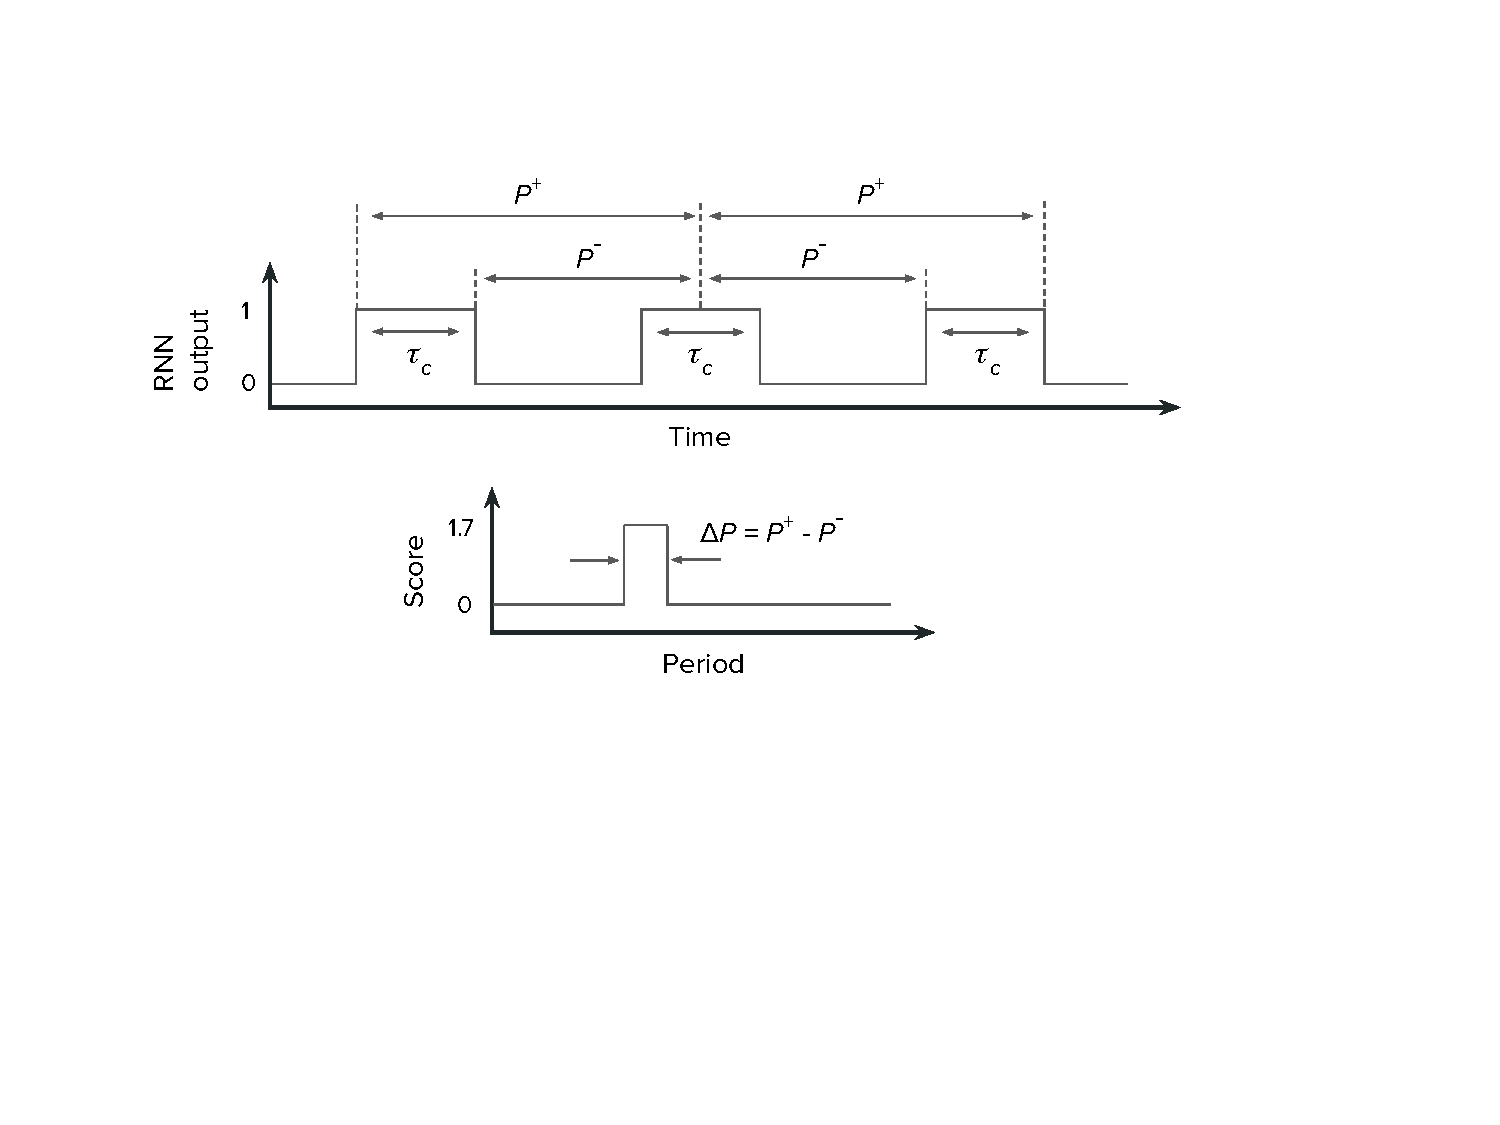
\includegraphics[width=0.6\linewidth]{Methodology/Figures/fold_drawing.pdf}
    \caption{An illustration of how the width $\Delta P$ of a peak in the periodogram relates to the duration $\tau_c$ of a signal. The PTS shown in the top shows $E=3$ potential events of a signal with a minimum and maximum period of $P^-$ and $P^+$. In this case, the candidate score for each value between $P^-$ and $P^+$ is the same in the periodogram shown below. For a number of events $E$ in the PTS, we have $\tau_c = (E-1)\frac{1}{2}\Delta P$, which in this case translates to $\tau_c = P^+ - P^-$.}
    \label{fig:fold_drawing}
\end{figure}
